%% ------------------------------------------------------------------------- %%
\chapter{Revisão de Literatura}
\label{cap:revisao}

	Para a realização deste trabalho, foi feita a pesquisa de termos relacionados à palavra usabilidade, para melhor entendimento dos conceitos citados nesta área, e de vários métodos existentes utilizados para avaliar a usabilidade em um ambiente específico, para aprimorar a escolha dos métodos a serem trabalhados nesta pesquisa. 
%% ------------------------------------------------------------------------- %%

\section{Conceitos de usabilidade}
\label{sec:conceitos}
	Antes de ser feita a avaliação quanto à usabilidade de um produto, é necessário compreender alguns conceitos relacionados ao tema para se evitar a falsa interpretação de diversos termos muito citados por diversos autores.

\subsection{Usabilidade}
\label{sec:usabilidade}
	Atualmente, este termo é amplamente utilizado devido à imensa quantidade de produtos que interagem com o ser humano, mas não possui uma única definição aceita por todos os pesquisadores da área. Segundo Carol Barnum \cite{barnum:01}, é preciso primeiramente identificar alguns significados errôneos para a palavra com o intuito de evitar falsas inferências, como ao afirmar que usabilidade é garantia de qualidade, ausência de defeitos, utilitário de funcionalidades de \emph{design} ou intrínseco em produtos. Ao contrário dessas más interpretações sobre o termo, Tullis et al. \cite{tullis:13} afirmam que, dentre todas as definições de usabilidade existentes, há algumas afirmações que se repetem:

\begin{itemize}
\item  um usuário está envolvido;
\item  esse usuário faz algo; e
\item  esse usuário faz algo com um produto, sistema ou outra coisa \cite{tullis:13}.
\end{itemize}
Essas afirmações podem ser vistas, por exemplo, nas definições abaixo:

\begin{itemize}
\item  Segundo a International Standarts Organization (ISO 9241-11), usabilidade é ``a medida pela qual um produto pode ser usado por usuários específicos para atingir objetivos específicos com eficácia, eficiência e satisfação em um contexto específico de uso''.
\item  Steve Krug \cite{krug:00} afirma que “Usabilidade realmente apenas significa ter certeza que algum produto funciona bem: que uma pessoa com habilidade e experiência na média (ou até abaixo da média) possa usar o produto - quer seja um site, um jato de combate, ou uma porta giratória - para sua finalidade sem ficar irremediavelmente frustrado.”
\end{itemize}

Com base nessas definições, pode-se afirmar que um produto com boa usabilidade não está imune a defeitos nem possui necessariamente alta qualidade, mas atende às expectativas do usuário sobre o produto, com eficácia, eficiência e satisfação. Apesar de a aceitação de um produto pelo usuário ser um fator bem importante para o sucesso do produto, muitos projetistas não dão o devido valor à avaliação da usabilidade, realizando-a apenas se houver tempo e recurso a mais que o planejado para o desenvolvimento do projeto \cite{anapaula12:MSc}. Isso se dá, entre outros motivos, pelo fato de programadores desenvolverem sempre funcionalidades em excesso por amarem tecnologia e serem curiosos quanto aos limites da ferramenta \cite{barnum:01}.

\subsection{Métricas de usabilidade}
\label{sec:metricas}
	Para serem processados dados quantitativos sobre a usabilidade de um produto, assim como no caso de algum fenômeno, são necessárias métricas para medir os dados obtidos. Tullis et al. \cite{tullis:13} afirmam que todas as métricas se baseiam em um sistema confiável de medição, pois utilizam o mesmo conjunto de medidas cada vez que algo é medido, no intuito de prover resultados comparáveis.

	No entanto, para medir a usabilidade, métricas específicas são utilizadas, conforme afirmam Tullis et al. \cite{tullis:13}: “Uma métrica de usabilidade revela algo sobre a interação entre o usuário e o produto: algum aspecto de eficácia (ser capaz de completar uma tarefa), eficiência (a quantidade de esforço exigido para completar a tarefa), ou satisfação (o grau de felicidade com sua experiência em que o usuário estava durante a realização da tarefa).” .  Em outras palavras, métricas de usabilidade, ao contrário da maioria das métricas, medem dados sobre atributos relacionados a pessoas.

	Segundo Tullis et al. \cite{tullis:13}, as principais métricas de usabilidade são: sucesso de uma tarefa, tempo para realização de uma tarefa, quantidade de erros, eficiência, capacidade de aprendizado, métricas baseadas em problemas, métricas de auto-relato, métricas comportamentais e psicológicas, métricas combinadas e comparativas, métricas de websites ao vivo e métrica de ordenação de cartões. O tipo de métrica utilizado neste trabalho serão as métricas baseadas em problemas de usabilidade, devido ao cenário descrito por Tullis et al. no qual esse teste se encaixa. O cenário escolhido será especificado na seção ~\ref{sec:metricas-usadas}, e o tipo de métrica selecionado  será detalhado a seguir.
\\
\subsubsection{Métricas baseadas em problemas}
\label{sec:metricas-problemas}

    Não há uma definição simples e clara sobre o que são problemas de usabilidade, mas uma definição possível é que são considerados problemas de usabilidade quaisquer estados do produto que prejudiquem a interação deste com o usuário e que, se alteradas, vão melhorar o software. Como exemplos de problemas, pode-se citar instâncias que: não permitem o sucesso de uma tarefa, como ao clicar em um link com conteúdo diferente esperado, estando na página principal, e ser redirecionado à mesma página; levam o usuário a sair do curso da tarefa, como ao existir links mais chamativos ao usuário que o link da tarefa inicial que ele desejava realizar; levam à falsa suposição do sucesso de uma tarefa, como ao não mostrar ao usuário uma falha ocorrida no processo de criação de um conteúdo; dentre outros \cite{tullis:13}.

    Apesar de muitos profissionais de usabilidade interpretarem problemas de usabilidade como dados puramente qualitativos e não os associarem a métricas, a medição destes problemas existe e auxilia bastante na melhoria do design do produto \cite{tullis:13}. Para medição dos problemas de usabilidade, é possível utilizar as seguintes métricas: frequência da quantidade de problemas, frequência de problemas por participante, frequência de participantes que identificam cada problema, classificação de problemas por categorias e classificação de problemas por tarefas \cite{tullis:13}.

As métricas baseadas em problemas que serão utilizadas nessa avaliação somativa são:
%Na  Figura~\ref{fig:chart-area} ***(mudar imagem)***, é possível ver quais métricas baseadas em problemas serão utilizadas nessa avaliação somativa. São elas:

\begin{itemize}
\item "classificação de problemas  por categorias"

Para facilitar a identificação e avaliação das falhas identificadas pelo usuário, é preciso separar em grupos.

\item "classificação de problemas por tarefas" 

Unindo as funcionalidades por tarefa, o usuário sente-se mais seguro para identificar eventuais falhas que ocorram, facilitando a comparação entre as funcionalidades.

\item "frequência de participantes que identificam cada problema". 

Com essa métrica, é possível, dentro do mesmo escopo, classificar facilmente as falhas de usabilidade.

\end{itemize}

O restante das métricas baseadas em problemas não poderá ser utilizado devido à insuficiência de dados disponíveis.

%\subsubsection{Métricas de relato do usuário}
%\label{sec:metricas-usuario}

%\subsection{Interação Humano-Computador}
%\label{sec:ihc}

%\subsection{Design centrado no usuário}
%\label{sec:dcu}
%	Barnum\cite{barnum:01} defende que o \emph{design} centrado no usuário “[...]é o processo de desenvolvimento do produto baseado em aprender sobre o usuário e em aplicar esse aprendizado para criar produtos que vão de encontro às necessidades dos usuários”  

%% ------------------------------------------------------------------------- %%

\section{Tipos de teste de usabilidade}
\label{sec:metodos-aplicacao}
    Como verificado na seção anterior, todos os termos relacionados com usabilidade envolvem o usuário, portanto é presumível que os testes de usabilidade sejam realizados com usuários do produto. No entanto, é preciso decidir qual o melhor momento para tal teste ser feito. Há dois tipos de testes que podem ser aplicados durante o processo de produção, chamados formativo e somativo, que serão descritos abaixo.

\subsection{Teste formativo}
\label{sec:teste-formativo}
%TODO: incluir cite%
    Este tipo de teste passou a ser mais utilizado com a importância de se reavaliar o que era modificado após um teste de usabilidade e de se avaliar a interação do usuário com novas funcionalidades. Além disso, é muito mais vantajoso a quem lança o produto que ele seja avaliado antes de seu lançamento, para evitar que usuários deixem de utilizar o produto por incontentamentos, mesmo que atualizações que corrijam o problema encontrado sejam implementadas posteriormente. 
    Com o intuito de suprir essas necessidades, o teste formativo é realizado de forma iterativa e frequente, e muitas vezes é incorporado ao processo de desenvolvimento, mais especificadamente, no desenvolvimento ágil. Quando em conjunto com este tipo de desenvolvimento, com a devida presença de profissionais em \emph{design}, é incluso em todas as fases de cada iteração do processo.
    Nas fases que antecedem o lançamento do produto, a avaliação da usabilidade é feita através de protótipos, pois o produto final para aquele lançamento ainda não está finalizado. Dentre os principais tipos de protótipos, pode-se citar os de papel, de \emph{powerpoint} e \emph{online}. 
    
%	foca na percepção do usuário de usabilidade e da sensação de satisfação; processo iterativo
%Usabilidade testada frequentemente, durante todo o processo de desenvolvimento; é indicado para incorporar no desenvolvimento ágil; exemplos de protótipos: papel, powerpoint, online (anapaula12:MSc); (barnum:01 121 e 124)

\subsection{Teste somativo}
\label{sec:teste-somativo}
    Quando usuários paravam de utilizar algum produto por frustrações ou faziam críticas negativas sobre ele, percebeu-se a importância de avaliar a usabilidade dos produtos. Porém, no princípio essa avaliação era feita tarde demais, depois que o produto já havia sido lançado ao mercado. Esse tipo de avaliação, realizado pós-lançamento, é chamado de teste somativo. 
    Ao contrário do teste formativo, ele é geralmente realizado apenas uma vez, para avaliar a eficiência do produto como um todo, tendo como base objetivos específicos \cite{barnum:01} como, por exemplo, avaliar a utilidade de determinadas funcionalidades no uso constante do produto pelos usuários. É importante notar que nele se faz necessária uma boa documentação dos erros encontrados na análise para correção posterior dos mesmos.
    Neste trabalho, este será o tipo de teste adotado, pois há um objetivo específico: avaliar e classificar a maioria dos problemas de usabilidade no sistema, através do cenário de descoberta de problemas.
    
%	antigamente mais usado; só uma vez
%	pra avaliar performance do produto com base em certos objetivos (barnum:01 122)
%	só implementar uma vez no tcc, pra avaliar a maioria das usabilidades (problem discovery); não dá continuidade, mas é um inicio
%	documentação se faz mais necessária pra contornar erros não corrigidos
	
%% ------------------------------------------------------------------------- %%

%\section{Métricas de avaliação}
%\label{sec:metricas-avaliacao}
%    Após a coleta dos dados, é necessária uma correta análise deles. Para tal, é importante não apenas distinguir os dados subjetivos dos objetivos, mas também evitar incoerências entre os dois tipos de dados \cite{barnum:01}, como ao se afirmar que uma funcionalidade é de fácil entendimento (dado subjetivo), mas demonstrar dificuldades ao realizar uma tarefa com este recurso (dado objetivo).
%    Neste trabalho, serão feitas análises quantitativas dos problemas de usabilidade avaliados.
%	barnum:01: fazer análise quantitativa dos problemas de %usabilidade; tomar cuidado com conflito entre dados subjetivos e objetivos; reunir também as críticas positivas
%TODO: procurar livro do Tullis%

%% ------------------------------------------------------------------------- %%



%% ------------------------------------------------------------------------- %%

%\subsection{�cidos Nucl�icos}\index{�cido!nucl�ico}\index{nucleot�deos}
%\label{sec:acidos_nucleicos}

%Na Figura~\ref{fig:humanbeta} texto texto texto texto texto texto texto texto

%\begin{figure}[!h]
%  \centering
%  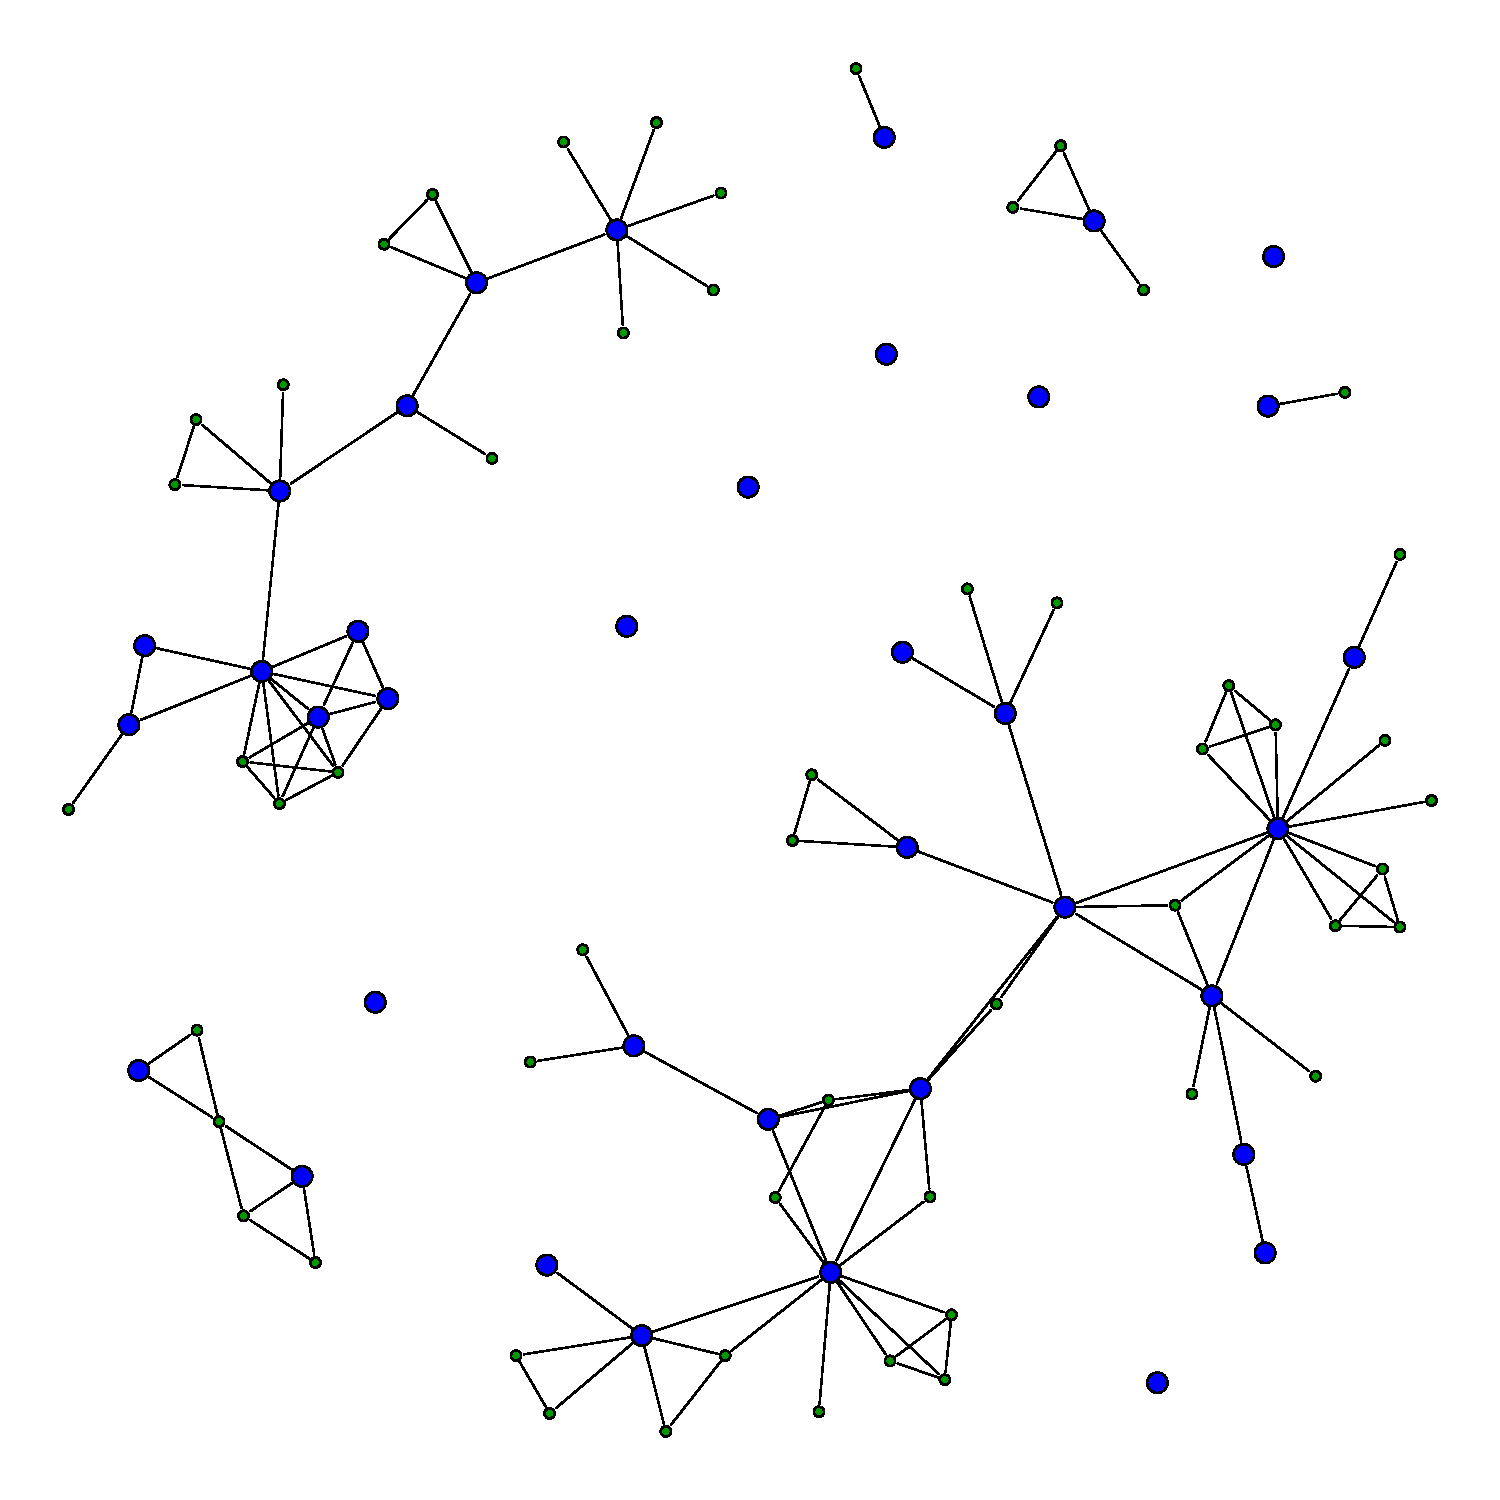
\includegraphics[width=.40\textwidth]{graph} 
%  \caption{Descri��o da figura mostrada.}
%  \label{fig:humanbeta} 
%\end{figure}

%% ------------------------------------------------------------------------- %%
%\subsection{Amino�cidos}\index{�cido!amino|(}
%\label{sec:amino_acidos}

%Veja na Tabela \ref{tab:amino_acidos}...  texto texto texto texto texto text
%\begin{table}[!t]
%\begin{center}
%    \begin{tabular}{c|c|l}
%	 \hline
%	 C�digo & Abreviatura & Nome completo \\ \hline
%    \texttt{A} & Ala & Alanina \\
%     \texttt{C} & Cys & Ciste�na \\
%     ...        & ... & ... \\
%     \texttt{W} & Trp & Tiptofano \\
%     \texttt{Y} & Tyr & Tirosina \\ \hline
%    \end{tabular}
%  \caption{C�digos, abreviaturas e nomes dos amino�cidos.}
%  \label{tab:amino_acidos}
%\end{center}
%\end{table}

% Foi utilizado o pacote listing para formatar c�digo fonte
% http://ctan.org/tex-archive/macros/latex/contrib/listings/listings.pdf
% Veja no preambulo do arquivo tese-exemplo.tex os par�metros de configura��o.

%\begin{lstlisting}[frame=trbl]
%    for(i = 0; i < 20; i++)
%    {
%        // Coment�rio 
%        System.out.println("Mensagem...");
%    }
%\end{lstlisting}


%% ------------------------------------------------------------------------- %%
%\section{Algumas Refer�ncias}
%\label{sec:algumas_referencias}

%� muito recomend�vel a utiliza��o de arquivos \emph{bibtex} para o gerenciamento
%de refer�ncias a trabalhos. Nesse sentido existem tr�s plataformas gratuitas
%que permitem a busca de refer�ncias acad�micas em formato bib: 
%\begin{itemize}
%	\item \emph{CiteULike} (patrocinados por Springer): \url{www.citeulike.org}
%	\item Cole��o de bibliografia em Ci�ncia da Computa��o: \url{liinwww.ira.uka.de/bibliography}
%	\item Google acad�mico (habilitar bibtex nas prefer�ncias): \url{scholar.google.com.br}
%\end{itemize}
%Lamentavelmente, ainda n�o existe um mecanismo de verifica��o ou valida��o das
%informa��es nessas plataformas. Portanto, � fortemente sugerido validar todas
%as informa��es de tal forma que as entradas bib estejam corretas.  Tamb�m, tome
%muito cuidado na padroniza��o das refer�ncias bibliogr�ficas: ou considere TODOS
%os nomes dos autores por extenso, ou TODOS os nomes dos autores abreviados.
%Evite misturas inapropriadas.
